\documentclass{standalone}
\usepackage{tikz}
\usetikzlibrary{positioning,decorations.pathreplacing}
\begin{document}
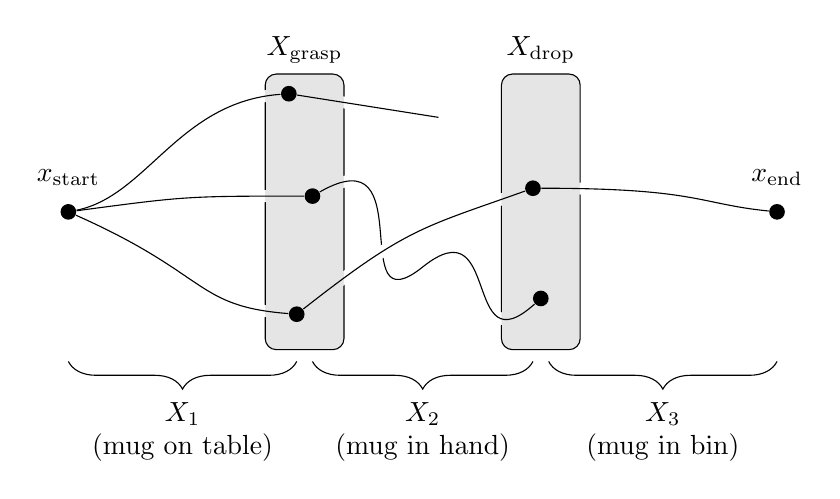
\begin{tikzpicture}
\node[draw,black,rounded corners,minimum height=3.5cm,minimum width=1cm]
   (Xgrasp) at (3,0) {};
\node[draw,black,rounded corners,minimum height=3.5cm,minimum width=1cm]
   (Xdrop) at (6,0) {};
\node[circle,fill=black,inner sep=2] (xstart) at (0,0) {};
\node[circle,fill=black,inner sep=2] (xg1) at (2.8,1.5) {};
\node[circle,fill=black,inner sep=2] (xg2) at (3.1,0.2) {};
\node[circle,fill=black,inner sep=2] (xg3) at (2.9,-1.3) {};
\node[circle,fill=black,inner sep=2] (xd1) at (5.9,0.3) {};
\node[circle,fill=black,inner sep=2] (xd2) at (6.0,-1.1) {};
\node[circle,fill=black,inner sep=2] (xend) at (9,0) {};
\node[above=0.1cm of xstart] {$x_{\mbox{\scriptsize start}}$};
\node[above=0cm of Xgrasp] {$X_{\mbox{\scriptsize grasp}}$};
\node[above=0cm of Xdrop] {$X_{\mbox{\scriptsize drop}}$};
\node[above=0.1cm of xend] {$x_{\mbox{\scriptsize end}}$};

\draw[line width=1.5mm,white]
   (xstart)
   .. controls (1,0.2) and (1.4,1.4) .. (xg1)
   -- (4.7,1.2);
\draw[line width=1.5mm,white]
   (xstart)
   .. controls (1.5,0.2) .. (xg2)
   .. controls (4.5,1) and (3.5,-1.5) .. (4.5,-0.7)
   .. controls (5.5,0.1) and (5.0,-2) .. (xd2);
\draw[line width=1.5mm,white]
   (xstart)
   .. controls (1.8,-0.8) and (1.6,-1.2) .. (xg3);

\draw
   (xstart)
   .. controls (1,0.2) and (1.4,1.4) .. (xg1)
   -- (4.7,1.2);
\draw
   (xstart)
   .. controls (1.5,0.2) .. (xg2)
   .. controls (4.5,1) and (3.5,-1.5) .. (4.5,-0.7)
   .. controls (5.5,0.1) and (5.0,-2) .. (xd2);
\draw[line width=1.5mm,white]
   (xg3)
   .. controls (4.3,-0.2) and (4.5,-0.2) .. (xd1)
   .. controls (8,0.3) and (8,0.1) .. (xend);
\draw
   (xstart)
   .. controls (1.8,-0.8) and (1.6,-1.2) .. (xg3)
   .. controls (4.3,-0.2) and (4.5,-0.2) .. (xd1)
   .. controls (8,0.3) and (8,0.1) .. (xend);

\node[fill,black,rounded corners,minimum height=3.5cm,minimum width=1cm,
   opacity=0.1] at (3,0) {};
\node[fill,black,rounded corners,minimum height=3.5cm,minimum width=1cm,
   opacity=0.1] at (6,0) {};

\draw [decorate,decoration={brace,mirror,amplitude=10pt}]
(0.0,-1.9) -- (2.9,-1.9) node [black,midway,yshift=-0.9cm,align=center]
   {$X_1$\\(mug on table)};

\draw [decorate,decoration={brace,mirror,amplitude=10pt}]
(3.1,-1.9) -- (5.9,-1.9) node [black,midway,yshift=-0.9cm,align=center]
   {$X_2$\\(mug in hand)};

\draw [decorate,decoration={brace,mirror,amplitude=10pt}]
(6.1,-1.9) -- (9.0,-1.9) node [black,midway,yshift=-0.9cm,align=center]
   {$X_3$\\(mug in bin)};

\end{tikzpicture}%
\end{document}
